%%
% 引言或背景
% 引言是论文正文的开端,应包括毕业论文选题的背景、目的和意义;对国内外研究现状和相关领域中已有的研究成果的简要评述;介绍本项研究工作研究设想、研究方法或实验设计、理论依据或实验基础;涉及范围和预期结果等。要求言简意赅,注意不要与摘要雷同或成为摘要的注解。
\chapter{绪论}
\label{chapter1: introduction}
%定义，过去的研究和现在的研究，意义，与现有结论的区别

\section{绪论}
\label{sec:background}
% What is the problem
% why is it interesting and important
% Why is it hards, why do naive approaches fails
% why hasn't it been solved before
% what are the key components of my approach and results, also include any specific limitations，do not repeat the abstract
%contribution
%引言是论文正文的开端，应包括毕业论文选题的背景、目的和意义；对国内外研究现状和相关领域中已有的研究成果的简要评述；创新点；介绍本项研究工作研究设想、研究方法或实验设计、理论依据或实验基础；涉及范围和预期结果等。要求言简意赅，注意不要与摘要雷同或成为摘要的注解。

\section{研究目的及意义}



\section{国内外研究现状和相关工作}


\subsection{接入机制设计}


\subsection{网络参数优化}

\subsection{物理层改进技术}



\section{本文研究目标与内容}


\subsection{本文创新点与主要贡献}



\section{论文结构安排}
\label{sec:arrangement}



%\begin{figure}[h]
%\centering 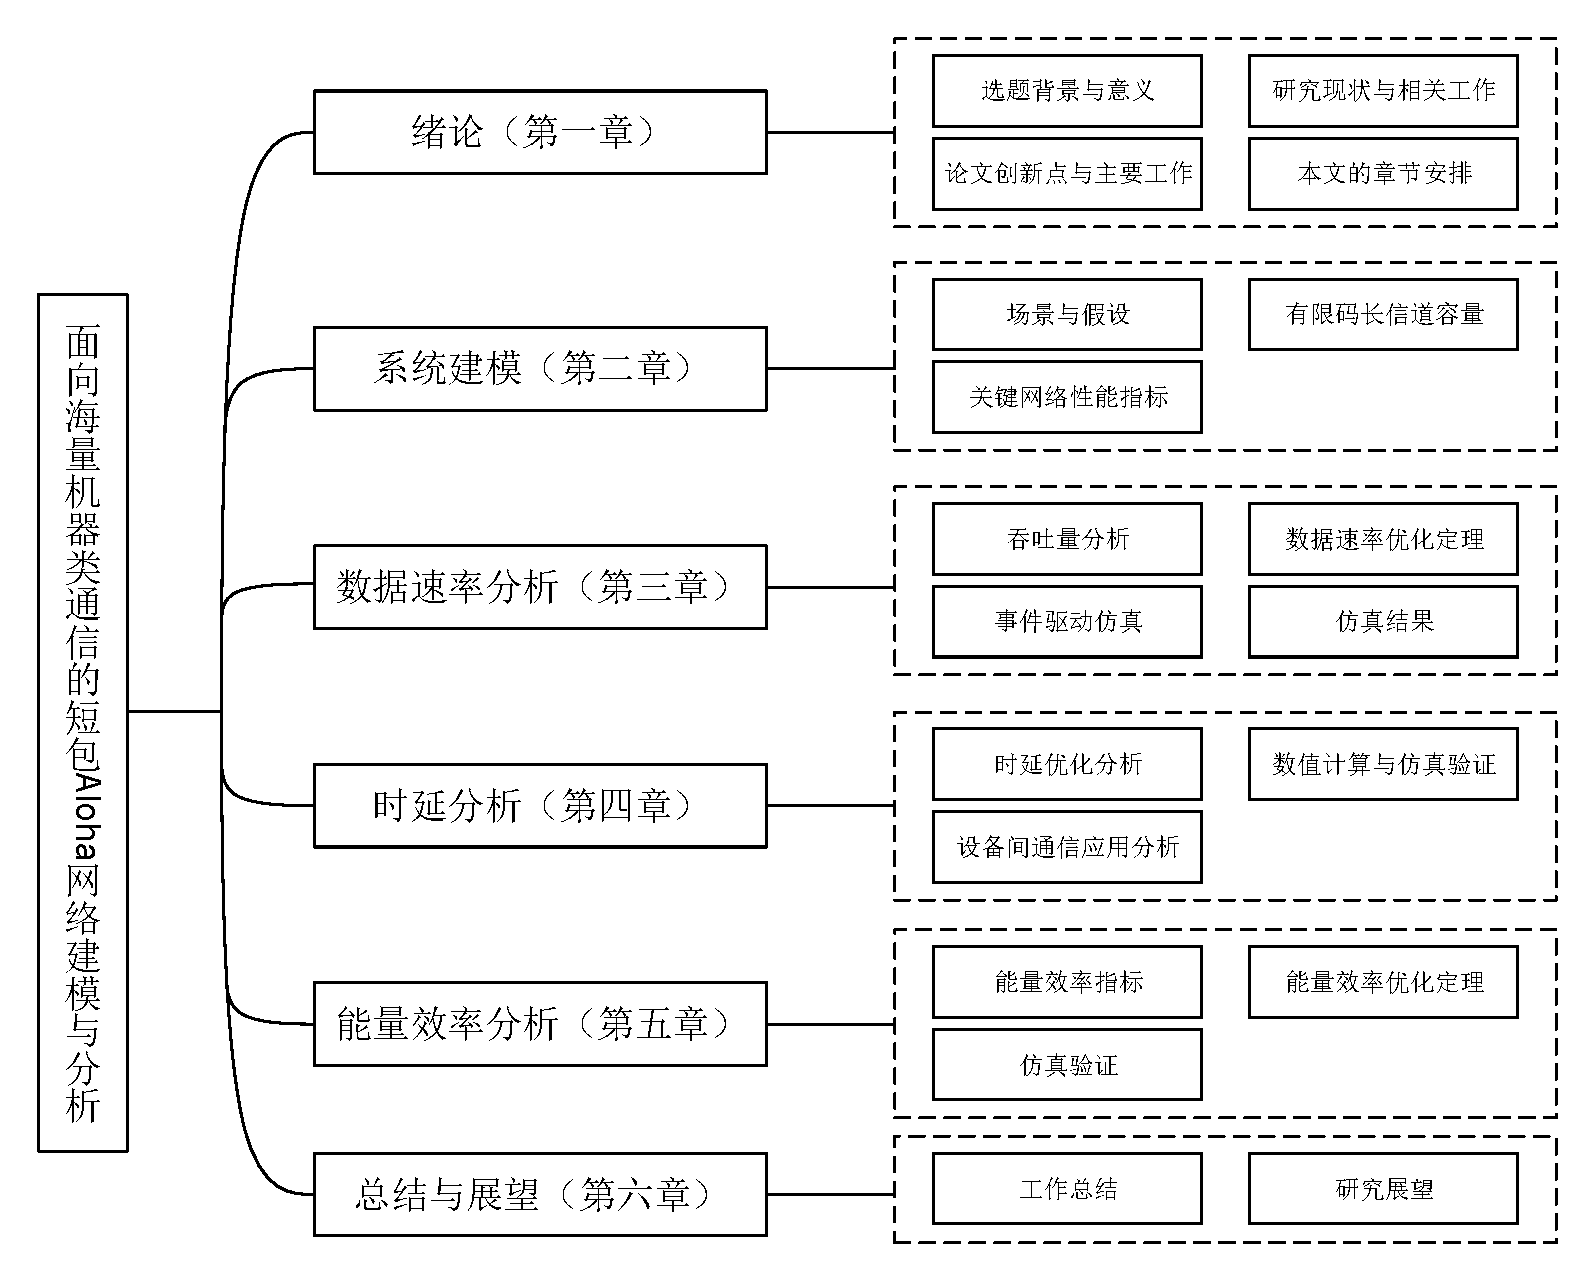
\includegraphics[angle=0,width=155mm,height=125mm]{image/weihua/structure.pdf}
%	\caption{论文章节安排}
%\label{fig:structure}
%\end{figure} 